\documentclass[letterpaper]{article}
\usepackage{amssymb}
\usepackage{fullpage}
\usepackage{amsmath}
\usepackage{epsfig,float,alltt}
\usepackage{psfrag,xr}
\usepackage[T1]{fontenc}
\usepackage{url}
\usepackage{pdfpages}
%\includepdfset{pagecommand=\thispagestyle{fancy}}
\author{Prof. Grizzle}
\title{Rob 501 - Mathematics for Robotics\\
HW \#9}

\begin{document}
\date{}
\maketitle


 \newcommand{\trace}{\mathrm{trace}}
\newcommand{\real}{\mathbb R}  % real numbers  {I\!\!R}
\newcommand{\nat}{\mathbb N}   % Natural numbers {I\!\!N}
\newcommand{\cp}{\mathbb C}    % complex numbers  {I\!\!\!\!C}
\newcommand{\ds}{\displaystyle}
\newcommand{\mf}[2]{\frac{\ds #1}{\ds #2}}
\newcommand{\Nagy}[2]{{Nagy, Page~#1, }{Prob.~#2}}
\newcommand{\spanof}[1]{\textrm{span} \{ #1 \}}
\parindent 0pt


\begin{flushright}
{\bfseries Due Nov. 29, 2018} \\
{\bfseries 3PM via Gradescope} \\[3mm]
\end{flushright}

\noindent \textbf{Remarks:}
 \begin{itemize}
 \item If you have been hearing about ``quadratic programs'' (QPs), well, Problem 2  is a simple case of a QP. You also solved one in HW 7 and in HW 1 (go back and look at Problem 6 of HW 1). We will do more advanced QPs at the end of the term.
     \end{itemize}


\begin{enumerate}


%Prob. 1   Under determined continued
\item Consider the finite dimensional vector space $({\cal X}, \real)$, where ${\cal X} = \spanof{1, t, t^2, \sin(\pi t)}$. Equip it with the inner product $<f,g>:=\int_{0}^2 f(\tau) g(\tau) d\tau$.  When working the problem, feel free to use MATLAB to compute any required integrals, and you may compute them symbolically or numerically, as you wish.
     \begin{enumerate}
\setlength{\itemsep}{.1in}
\renewcommand{\labelenumi}{(\alph{enumi})}
\item Find the vector of minimum norm that satisfies $<f, t>=2$.

\item  Find the vector of minimum norm that satisfies $<f, t>=2$ and $<f,\sin(\pi t)>=\pi$.

\end{enumerate}

%Prob. 2   Under determined continued
%\item \textbf{Magic Equations for Under Determined Equations:\footnote{By the way, I just called them that in class and it kind of stuck. No one else uses this vocabulary. Recall that the first time we saw equations like these in the over determined case, I just said, ``hey, this is the answer.'' They did seem like ``magic'', so I called them that. It was only later that I gave you a proof. Then it was science and not magic!}}
\item \textbf{Underdetermined Equations:} We consider
 $Ax=b$,
    where $b\in \real^p$, $x\in \real^n$, $n>p$.   Use the normal equations derived in HW \#8  to solve the following problems. The key is to interpret the rows of $Ax=b$ in terms of inner product conditions that look like $<x,y_i> = c_i$.
     \begin{enumerate}
\setlength{\itemsep}{.1in}
\renewcommand{\labelenumi}{(\alph{enumi})}
\item We assume an inner product on $\real^n$ defined by $<x,z>:= x^\top z,$
 and thus $||x|| = (x^\top x)^{1/2}$.  Show that if the rows of $A$ are linearly independent, then
    $$\widehat{x}:= \mathrm{arg}~\min_{Ax=b} ||x||$$
    is given by $ \widehat{x} = A^\top \left( A A^\top \right)^{-1}b$

\item  We assume an inner product on $\real^n$ defined by $<x,z>:= x^\top Q z,$
    where $Q \succ 0$, and thus $||x|| = (x^\top Q x)^{1/2}$.  Show that if the rows of $A$ are linearly independent, then
    $$\widehat{x}:= \mathrm{arg}~\min_{Ax=b} ||x||$$
    is given by $ \widehat{x} = Q^{-1} A^\top \left( A Q^{-1} A^\top \right)^{-1}b$.

\end{enumerate}

\textbf{Remark:} A QP is an optimization problem of the form $$\widehat{x}:= \underset{ \begin{array}{l} A_{eq} x=b_{eq} \\A_{in} x \le b_{in} \end{array} } { \mathrm{arg}~\min}||x||^2.$$ The key addition is that inequality constraints, $A_{in} x \le b_{in}, $ can also be included. We'll talk more about this the last day of lecture.

%Prob. 3
% Compute QR of a matrix. Solve it that way. Compare to MATLAB.
\item  We did one version of the QR factorization in lecture (we assumed $A$ had linearly independent columns). Scan MATLAB's documentation of the \texttt{qr} function and note its \textit{economy} version, \texttt{[Q,R]=qr(A,0)}. Using Gram Schmidt, compute the QR factorization of the matrix $A$ below ``by hand'' (you can do any vector multiplications and such in MATLAB\footnote{This is just to encourage you to do one QR factorization yourself without relying on MATLAB's built-in function.}). Compare your answer to MATALB's \texttt{[Q,R]=qr(A)} and  \texttt{[Q,R]=qr(A,0)} and discuss similarities and differences.
    $$ A=\left[ \begin{array}{rr}  1&   2 \\   3 &  4 \\  5&   6\end{array} \right]$$

%   >> [Q,R]=qr(hilb(8));
%>> M=hilb(10);[Q,R]=qr(M);
%>> inv(R)*Q'*M
%
% inv(M)*M


%Prob.4
\item The following problem arises in camera calibration: $$\widehat{x} = \text{arg}~\min_{x^\top x=1} x^\top A^\top A x.$$ Show that if $A$ is real\footnote{When we write down \texttt{arg~min}, we should also have conditions so that the answer is unique. For this problem, we need the smallest e-value of $A^\top A$ to be unique, and even then, it is only unique up to a sign (i.e., if $\widehat{x}$ is an answer, then so is $-\widehat{x}$). Unfortunately, in the literature, you typically see the problem given as stated.}, then $\widehat{x}$ is given by the last column of $V$ where $A=U \Sigma V^\top$ is the SVD of $A$.

%%Prob 6
%\item Compute a rank 2 approximation of $$A=\left[ \begin{array}{rrr}4.041& 7.046& 3.014\\10.045& 17.032& 7.027\\16.006& 27.005& 11.048\end{array} \right].$$
%    That is find $\widehat{A} =\text{arg}~\min_{\text{rank}~ B = 2} ||A - B||_2$, where the matrix norm being used is
%    $$||M||_2 = \sqrt{\lambda_{max}(M^\top M)}$$

%Prob 5
\item Compute a rank 2 approximation of $$A=\left[ \begin{array}{rrr}4.041& 7.046& 3.014\\10.045& 17.032& 7.027\\16.006& 27.005& 11.048\end{array} \right].$$
    In particular, find $\Delta A$ of smallest norm such that $\widehat{A}:=A+\Delta A$ has rank 2. The matrix norm being used is
    $$||M||_2 = \sqrt{\lambda_{max}(M^\top M)}.$$ It is enough to give $\widehat{A}$, the rank 2 approximation, in your solution.


%Prob 6: Image compression %Use SVD for something cool.
\item This problem is just for fun. It will not show up on any exam. Download the file \texttt{zebra.jpg} from the MATLAB folder. Everything I know about image compression, I learned in 15 minutes with a google search\footnote{You might also try the last page of \url{http://persson.berkeley.edu/18.335/lec3handout2pp.pdf} and glance at \newline \url{http://www.math.ucla.edu/~wittman/PCMI/pcmi1.pdf}} on ``image svd''. I invite you to do the same! These commands show how you can read an image into MATLAB, covert it to double precision arithmetic, perform a numerical operation on the matrix, convert it back to binary grey scale, and print it to a figure:
    \begin{verbatim}
A = imread('zebra.jpg');
%throw away color information for this example
A=A(:,:,1);
% show the image
figure(1)
imshow(A)
%convert to double precision
B=double(A);
%Let's do a matrix operation; you will find something more imaginative to do
C=fliplr(B);
%convert back to binary
C=uint8(C);
%show the image
figure(2)
imshow(C)
    \end{verbatim}
         \begin{enumerate}
\setlength{\itemsep}{.1in}
\renewcommand{\labelenumi}{(\alph{enumi})}
\item Use the SVD to produce a low-rank approximation to the image and display it. Can you reduce the rank by 75\% and still have an acceptable image? Less? No, need more? The purpose is to illustrate visually that the SVD can help you to find and eliminate redundant data. Turn in the original image and your low rank approximation; state the rank of your approximation.

\item  Download a ``wholesome'' image\footnote{Be considerate! Animals and scenery tend to be non-controversial.} from the internet and repeat the above.

\end{enumerate}

%Prob 7
\item Estimating derivatives of functions numerically. In this problem, we introduce a method to estimate the Jacobian of a function numerically.

                \begin{enumerate}
\setlength{\itemsep}{.1in}
\renewcommand{\labelenumi}{(\alph{enumi})}
\item Compute the Jacobian of the following function $f:\real^3 \to \real$ analytically and  evaluate it at the point $x^*=[1 ~3~ -1]^\top$
 \begin{equation}
    \label{equation1}
    f({x_1} , {x_2} , {x_3})=3{x_1}\left[2{x_2}-({x_3})^3 \right]+ \frac{({x_2})^4}{3}.
\end{equation}
Recall that the gradient of a scalar valued function is normally written as a row vector
$$ \frac{\partial f (x)}{\partial x}:=[  \frac{\partial f(x)}{\partial x_1}~~ \frac{\partial f(x)}{\partial x_2}~~ \frac{\partial f(x)}{\partial x_3}].$$

\item In calculus, you learned that $ \frac{\partial f(x^*)}{\partial x_i}:=\lim_{\delta \to 0} \frac{f({x}^*+ \delta {e}_i)- f({x}^*)}{ \delta}$, where ${e_i} ,\: i=1:3$ are the natural basis vectors, and thus, for a fixed $\delta>0$, you might estimate the derivative by
    $$ \frac{\partial f(x^*)}{\partial x_i} \approx \frac{f({x}^*+  \delta {e}_i)- f({x}^*)}{ \delta}$$
    It turns out that better numerical accuracy is usually obtained by a \textit{symmetric difference}\footnote{It can be shown that a symmetric difference is EXACT for a quadratic function. You might want to try that out.}
\begin{equation}
 \label{equation2}
\frac{\partial f(x^*)}{\partial x_i} \approx \frac{f({x}^* + \delta {e}_i)- f({x}^* - \delta {e}_i)}{2  \delta}.
\end{equation}
Compute a numerical approximation to the Jacobian of the function \eqref{equation1} using symmetric differences and report the value(s) you used for $\delta$. You are not obliged to use the same $\delta$ for each partial derivative. Use the same $x^*$ as in part (a).


\item When you already know the answer, it is easy to play with $\delta$ and come up with a good numerical approximation to the derivative. What will you do when you do not know the answer before hand? Let's find out! Download the function \texttt{funcPartC.p} from the MATLAB folder. It is a hidden function $f: \real^5 \to \real$. Report its Jacobian at ${x^*}=[1, 1, 1, 1, 1]$.

    Here is how to call the function
    \begin{verbatim}
    x0=[1 2 3 4 5];
    f=funcPartC(x0)
    f = 2.1281e+01
    \end{verbatim}

\end{enumerate}
\newpage
%Prob 8 - Kalman Filter one step
\item \textbf{One step update of a robot's state using a Kalman filter}. You are given a simple robot that moves in one dimension, say along the $X$-axis. \\
\begin{figure}[h]
	\centering
	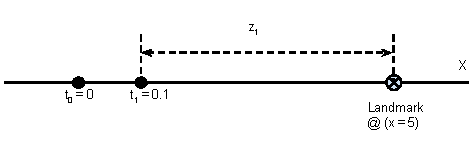
\includegraphics[width = 0.7\linewidth]{kalman_filter.pdf}
	\caption{\label{robot_ref_frame}Robot's motion is along the $X$-axis. The landmark is a fixed point at $x=5$m.}
\end{figure}

Your robot starts at a position\footnote{We have used the notation, $x \sim \mathcal{N}(\mu, \Sigma)$, in previous HW sets.} $x_0$, which is normally distributed $x_0 \sim \mathcal{N}(1, 0.25)$, i.e. $\mu_0 = 1$ and $\Sigma_0=\sigma^2= 0.25$. The state of your robot at the next time step is given by the following equation
\begin{align}
	x_{1}= x_0 + u_1 \cdot \delta_t~~\text{(state propagation model)}\label{equation3}
\end{align}
where $u_1$, the action taken, is also normally distributed\footnote{Why would the control signal be random? Well, what if the feet or the wheels of your robot are slipping in sand or wet grass? Then the control signal you command to the motor is not the action that will be applied to the body of the robot!}, $u_1 \sim \mathcal{N}(10,16)$, i.e. $\hat u_1 = 10$, $R=16$ and $\delta_t=0.1$ is the time step. \\

Fortunately, your robot has a reasonably accurate time of flight sensor\footnote{Understanding how LiDAR works https://www.youtube.com/watch?v=EYbhNSUnIdU. More information about LiDARs specifically  in mobile robots can be found here, https://www.clearpathrobotics.com/2015/04/robots-101-lasers/} which can measure the robot's distance from a fixed landmark. Based on the physics of the situation, you expect the output of your robot's sensor (i.e., the measurement) to be related to the robot's position by
\begin{align}
\hat z_t= \frac{2}{c}{(5-x_t)},
\end{align}
where $x_t$ is the robot's position at time $t$, $c$ is the speed of light\footnote{Use $c = 3\times 10^8$ m/s} and $\hat z_t$ is the corresponding expected output\footnote{The expected output, $\mathbb{E}\{z\}=\mu_z$, is the mean value}(in seconds) from the sensor.\\

Because your sensor is a real device, it has error in its measurement; the actual sensor output is modeled to be, $z_1 \sim \mathcal{N}(\hat z_t, Q)$, where $Q$ is the uncertainty in the measurement. In this case, the manufacturer tells you that your LiDAR has uncertainty, $Q=10^{-18}$.

\textbf{Problem:} Suppose at time $t=0.1s$ your robot takes action $u_1$ and moves according to \eqref{equation3}. Your sensor outputs  $z_1 = 2.2 \times 10^{-8}$s. Estimate the position $x_1$ of your robot at time $t=0.1$ and the uncertainty in its position. Give your answer in the form of a normal distribution $ x_1 \sim \mathcal{N}(\mu_1, \Sigma_1)$.

%   \begin{verbatim}
%Estimate derivatives numerically
%
%1) Symmetric difference  [f(x+delta e_i) - f(x-delta e_i) ]/ (2 delta)
%
%2) Fit Ax+b to function values.
%
%   \end{verbatim}

%End of list of HW Problems
\end{enumerate}

\newpage

\begin{center}
{\bf Hints}
\end{center}
\noindent \textbf{Hints: Prob. 1 } Apply Problem 6 from HW \#8. You may enjoy the symbolic toolbox for doing the calculations.
\begin{verbatim}
syms t pi
f=t^2;
g=exp(pi*t);
a=0; b=2;
G11=int(f*f,a,b);
G11=simple(G11)
\end{verbatim}
Commands such as \texttt{inv} and \texttt{numden} work in the symbolic toolbox. Also checkout \texttt{simplify} and \texttt{pretty}.

\vspace{1cm}
\noindent \textbf{Hints: Prob. 2 }  Decompose $A$ by its rows,
 $$A= \left[\begin{array}{c} a_1 \\ a_2 \\ \vdots \\ a_p\end{array} \right].$$
Define $\tilde{A} = A Q^{-1}$ (why is $Q$ invertible?), and define $v_i \in \real^n$ by
$$v_i = (a_i Q^{-1})^\top = Q^{-1} a_i^\top,$$
where we have used the fact that $Q$ is symmetric. Show that
$$Ax=b \Leftrightarrow <v_i,x> = b_i,~~  1\le i \le p.$$
Now, work out those normal equations from last week! If the above derivation confuses you, set $Q=I$ and you will get it! That is why I broke the problem into two parts.\\

\textbf{Remark:} Squaring the norm does not change the answer\footnote{Yes, the value is squared, but the argument achieving the minimum, i.e., the $\widehat{x}$, does not change.} to the optimization problem because it is a strictly monotonically increasing function.
 $$\widehat{x}:= \mathrm{arg}~\min_{Ax=b} ||x|| =  \mathrm{arg}~\min_{Ax=b} ||x||^2= \mathrm{arg}~\min_{Ax=b} x^\top Q x.$$
The corresponding QP is always written using the form on the right.

\vspace{1cm}

\noindent \textbf{Hints: Prob. 3 } Nothing exciting here. Just pointing out that there exist multiple versions of the QR factorization.

\vspace{1cm}

\noindent \textbf{Hints: Prob. 4 } We have seen this problem before. Recall HW \#2, Prob. 7-(b). How does  the e-vector of $A^\top A$ corresponding to the minimum e-value relate to the columns of $V$? (See statement of SVD Theorem given in lecture).

\vspace{1cm}

\noindent \textbf{Hints: Prob. 5 } See the handout SVD\_Rob501 in the resource folder...the one everyone slept through! If this were not very useful and practical stuff, I would not pester you about it. I know, about this point in the term, everyone is pretty tired.

\vspace{1cm}

\noindent \textbf{Hints: Prob. 6 } \texttt{ k=YourValue; C=U(:,1:k)*S(1:k,1:k)*V(:,1:k)';} Too much said. The problem is for fun, but the message is interesting!

\vspace{1cm}

\noindent \textbf{Hints: Prob. 7 } Oh, the age-old problem, how to tune parameters in algorithms? In this case, a \textit{rule of thumb} is, if decreasing $\delta$ by a factor of 2 does not significantly change the estimate, then you can stop.\\

\noindent \texttt{Remark on exactness for a quadratic function:} Let $f(x) = ax^2 + bx + c$   be a quadratic. Performing the symmetric difference quotient about a point $x^*$, we have

\begin{align*}
\frac{f(x^*+h) - f(x^*-h)}{2h} &= \frac{a(x^*+h)^2 +b(x^*+h) + c - (a(x^*-h)^2 +b(x^*-h) + c)}{2h} \\
&= \frac{a{x^*}^2 + 2ax^*h + ah^2 + bx^* + bh + c - a{x^*}^2 + 2ax^*h - ah^2 - bx^* + bh - c}{2h} \\
&= \frac{4ax^*h + 2bh}{2h} \\
&= \frac{2h(2ax^* + b)}{2h} \\
&= 2ax^* + b,
\end{align*}
where we recognize the last line as the derivative at $x^*$.

\vspace{1cm}

\noindent \textbf{Hints: Prob. 8 } You have all the values for the Kalman filter available to you. Recall that you have seen in the handout on Gaussian Random Variables that if $x_1$ and $x_2$ are uncorrelated and $Y=Ax_1 + Bx_2$, then
\begin{align}
	\mu_y= A \mu_{x_1} + B \mu_{x_2} \nonumber \\
	\Sigma_y = A \Sigma_{x_1} A^\top + B \Sigma_{x_2} B^\top \nonumber
\end{align}
In this problem, you can see that $A=1$ and $B=0.1$, which will allow you to compute $\hat x_{1|0}$ and $P_{1|0}$. The rest of the data is available to you. Plug the values into the Kalman filter equations and note that you want to compute $\hat x_{1|1}$ and $P_{1|1}$, i.e. $x_1 \sim \mathcal{N} (\hat x_{1|1},P_{1|1})$\\

\textbf{Kalman Filter Equations with action model:}\\
\textit{Prediction Step:}
\begin{align}
	\hat x_{k+1|k}= A \hat x_{k|k} + B \hat u_{1} \nonumber \\
	P_{k+1|k} = A P_{k|k}  A^\top + B R  B^\top \nonumber
\end{align}
\textit{Measurement Update Step:}
\begin{align}
	K_{k+1} = P_{k+1|k} C^\top(C P_{k+1|k} C^\top + Q)^{-1} \nonumber \\
	\hat x_{k+1|k+1}= \hat x_{k+1|k} + K_{k+1}(z_{k+1} - \hat z_{k+1|k}) \nonumber \\
	P_{k+1|k+1} = P_{k+1|k} -  K_{k+1} C P_{k+1|k} \nonumber
\end{align}
$\hat z_{k+1|k}$ is the expected output if the position and measurement were not stochastic, i.e. using (4),   $$\hat z_{k+1|k} = \frac{2}{c}(5-\hat x_{k+1|k})$$
\end{document}


